\chapter{Evaluation}\label{Evaluation}

	\section{Requirement analysis}
	In this section I will go over the requirements that were made before the beginning of the project (\ref{requirements}) 
	and showcase how each of them are satisfied.

	The backend of the application is scalable in several ways. The most obvious one, is how the application is deployed on AWS. 
	If the resource usages hit a certain treshold, a new task is deployed. If the task cannot fit on an already running EC2 instance,
	the running EC2 instances scale up. This was desribed in section \ref{awsdeploy}. The other way the application supports 
	scalability is the way it handles multiple generation requests. Both the server (\ref{Generator Server}) and the client
	(\ref{Generator Client}) for the generator 
	functionality support multithreaded operation. As a result, generation requests can run in parallel, and the resource utilization
	is improved.

	The generation can be cancelled. The backend sends cancellation requests to the generator server (\ref{clientcancel}).
	When the generator server receives a cancel request (\ref{serverendpointcancel}), it instructs the dispatcher 
	(\ref{servercanceldispatcher}) to cancel the generation on the executor (\ref{serverexecutorcancel}).

	The frontend is able to show the state of the model generation. The states are sent by the generator server's executor via
	the open session to the clients.

	There is a timeout set for both the backend generator client and the generator server. This insures that even if some kind of 
	unexpected operation happens, the generation will not be stalled and use resources in a locked state.

	The editor and the generator can be deployed together. During development phase, the backend and the generator server can be 
	deployed together, via the gradle "run" task. This starts running both the generator microservice and the backend locally.
	Other than that a docker compose (\ref{Docker images}) file was written, so that the containerized applications can be run locally.

	One optional requirement was not satisfied by this implementation. The creation of other type of clients other than the browser
	based one is possible, but tedious. My testing python script basically acts as a different client, but it replicates the WebSocket
	messages of the frontend client, in order to create an editing session and send generation requests.

	The price of the hosting has changed due to the issues described in \ref{ALB NAT}. The price of the deployment for an hourly rate 
	is expected to be:

	\begin{center}
		Minimum cost per hour = $2 \times \$0.0108$ + $2 \times \$0.02394$ = \$0.06948
	\end{center}

	\section{Benchmarks} \label{Benchmarks}
		\subsection{Test methodology}
		I wrote a Python script replicating the WebSocket messages of the Refinery frontend. First it creates the connection
		towards the server. Then sends the initial update
		of the example text, that can be seen in the editor at start. Then a generation request is sent to the backend and the start time of the generation
		is logged. When all of the generation results have arrived and none of them is an error, the end time of the generation is logged. 
		The script is implemented in a way, where it can run in a multithreaded way. I can send out as many simultaneous generation requests 
		from as many python clients as I would want to. In the tests, I sent out 1, 25, 50, 75, 100, 125, 150, 175, 200, 225 generation requests
		at the exact same time, and analyzed how the response times changed.

		The response times were exported to a JSON file at the end of each test. I used python's matplotlib library to visualize the results
		of each test.

		The running of the python test client could be done on an Amazon EC2 instance or on a personal computer. I have decided to run the test 
		from my own personal computer, as this provides a more accurate representation of the real usage of the application.

		\subsubsection{External threats to validity}
			Since the infrastructure is deployed on Amazon's infrastructure, the availability of the service and the communication speeds between the two services 
			depend on Amazon's network. As the results cannot be 100\% accurate, repeated testing should be
			performed.

			The network speeds are not constant and can be very volatile during the period of the test. The upload and download speeds of my computer, running the 
			python test client can also make some test data dirty / invalid.  Repeated testing should also solve this threat.

		\subsection{Results}
			\subsubsection{First test (Generations with one allocated thread)} \label{firsttest}
			The purpose of this test was to compare the old implementation with the new one in terms of response times. This was 
			the default deployment of the old implementaiton.

			The tests were performed with two t3.micro EC2 instances running at the start. These VMs have 2vCPUs and 1GB of memory. I allocated
			2vCPUs and 0.9GBs of memory for each task. Since I was running two services, with the forementioned task configurations, 
			those would not be able to fit on a single EC2 instance. The auto scaling acted accordingly, and deployed the services on two 
			separate EC2 instance. 

			The "REFINERY\_MODEL\_GENERATION\_THREADS" environment variable was not set in the task configurations. As a result, the tasks ran with only 1 thread
			allocated for the model generation requests.
			This is the default setting of for the deployment, and the old implementation is deployed in production with this setting.

			The results can be seen in figure \ref{1threadold} and figure \ref{1threadnew}:

			\begin{figure}[h!] 
				\begin{center}
					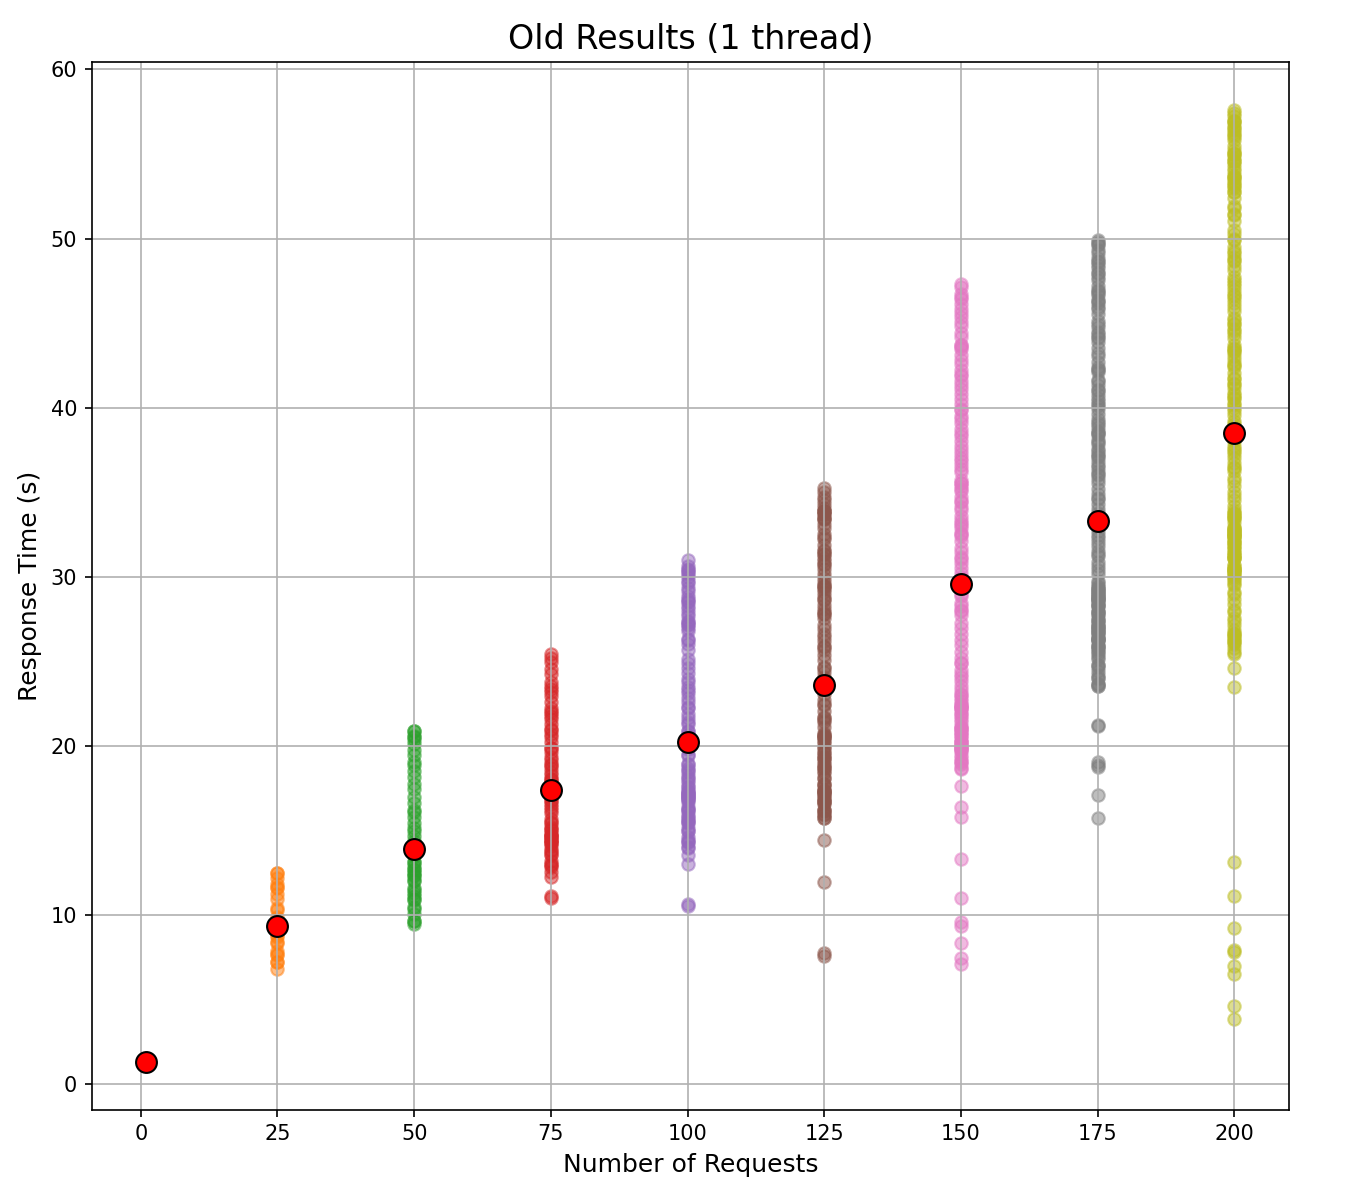
\includegraphics[scale=0.6]{include/imgs/1thread_old.PNG}
					\caption{Generation requests with the old implementation}
					\label{1threadold}
				\end{center}
			\end{figure}

			With only 1 thread being allocated the response times did not improve. This comes down to the queueing mechanism of the dispatcher at the client side.
			Even though our generator server could handle multiple simultaneous generations, the client applies a queue for the sending out of the generation requests.
			That can also be seen in the results. The response times grew in a linear fashion.

			\begin{figure}[h!] 
				\begin{center}
					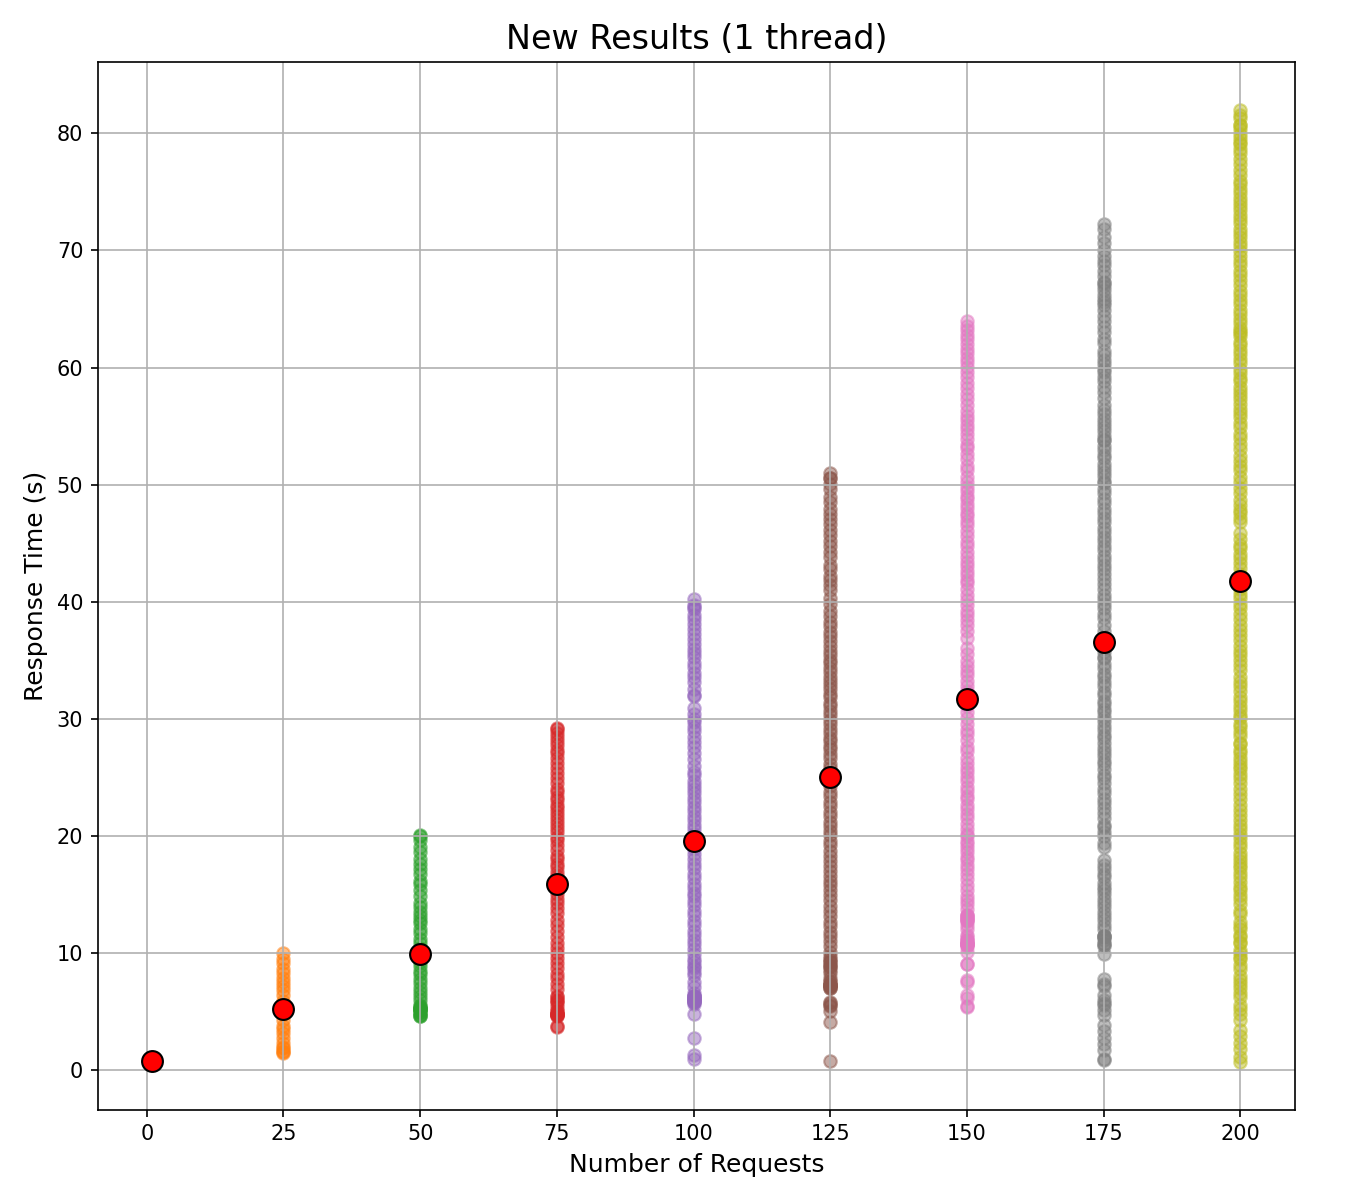
\includegraphics[scale=0.6]{include/imgs/1thread_new.PNG}
					\caption{Generation requests with the generation runnning on the microservice}
					\label{1threadnew}
				\end{center}
			\end{figure}

			This is due to the nature in which the architecture is implemented. If the generation client in the backend only (section \ref{Generator Client})
			uses one thread for sending out the 
			generation requests, the advantages of the multithreaded working in the generator server (section \ref{Generator Server}) cannot be utilized. 
			If the multithreaded working is not used, the response times 
			can only become worse, as there is an extra layer of networking communication added to the process. 

			\pagebreak
			\subsubsection{Second test (Generations with four allocated threads)}\label{testtwo}
				The purpose of this test was to compare the old implementation with the new one in terms of response times. This was 
				deployment utilized the multithreaded nature of the generator server, by using four threads for model generation.

				These tests were performed with two t3.micro EC2 instances running at the start. These VMs have 2vCPUs and 1GB of memory. I allocated
				2vCPUs and 0.9GBs of memory for each task. 

				The "REFINERY\_MODEL\_GENERATION\_THREADS" environment variable, contrary to the test in \ref{firsttest}, was set in the task configurations. 
				I set the value of it to be 4. I chose 4, because the t3.micro EC2 instances each have 2 vCPUs with 4 computational threads.

				The results were as follows:

				\begin{figure}[h!] 
					\begin{center}
						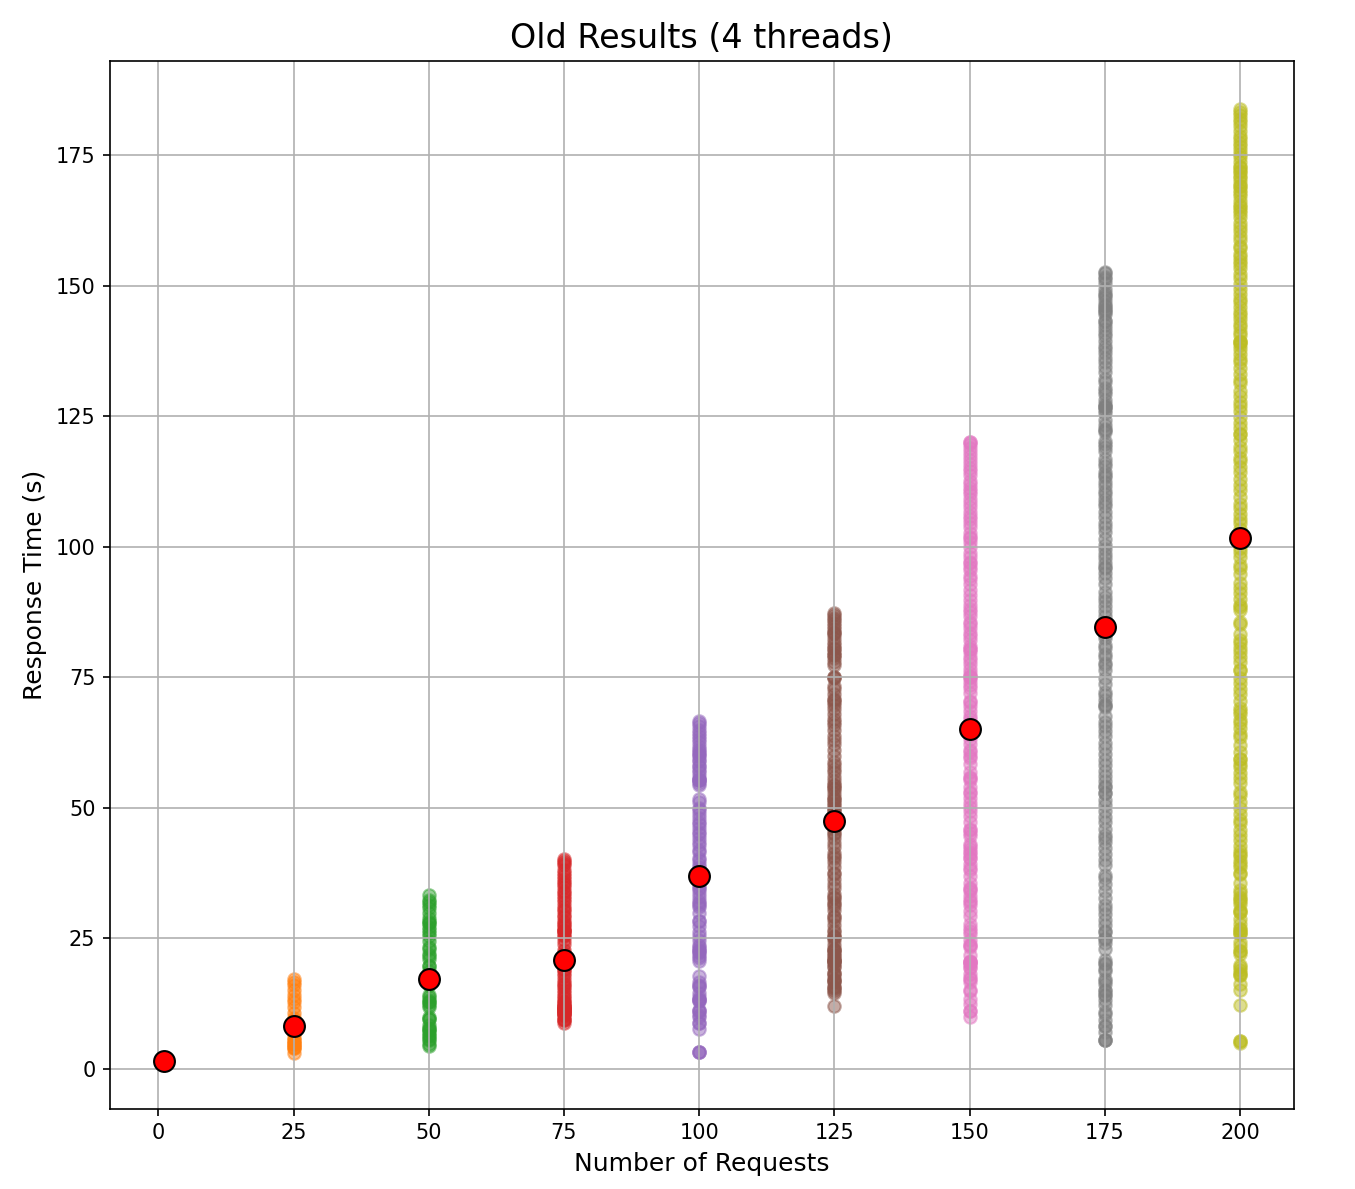
\includegraphics[scale=0.6]{include/imgs/4threads_old.PNG}
						\caption{Generation requests with 4 threads, old implementation}
						\label{4threadsold}	
					\end{center}
				\end{figure}

				The results in figure \ref{4threadsold} indicate, that the model generation running in a true multithreaded fashion slows down the old implementation. The 
				deviation of the response times is much bigger, compared to the results of running on a single thread. Both the medians and the maximum of the response times
				grow in an exponential way.

				\begin{figure}[h]
					\begin{center}
						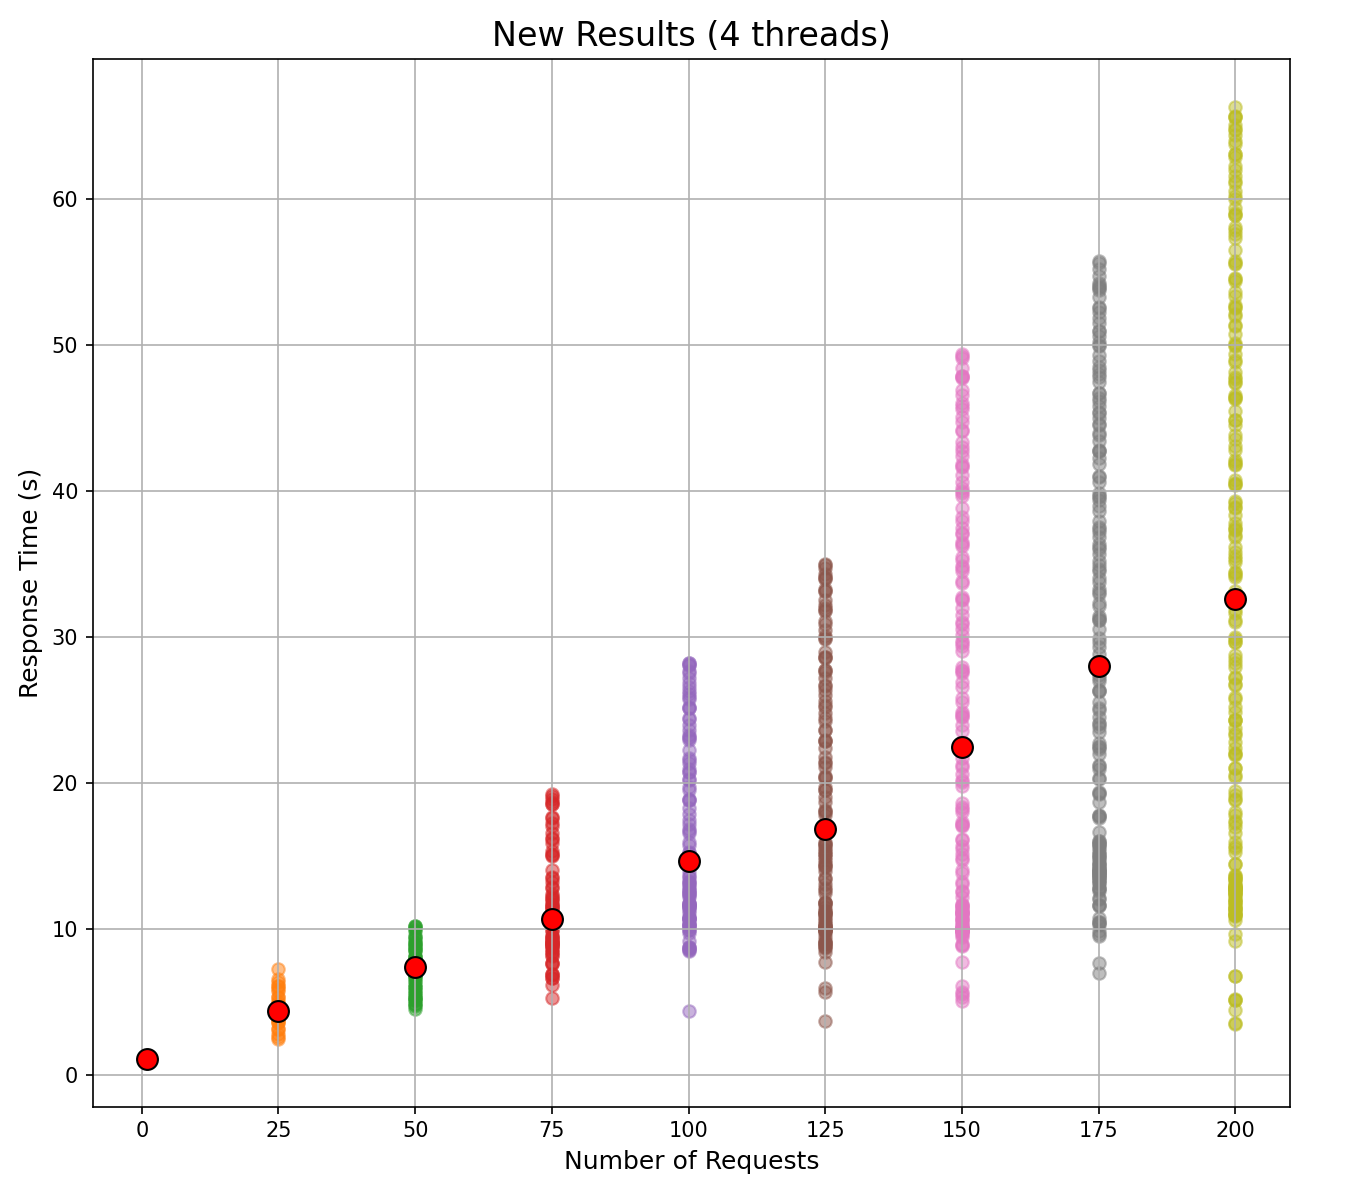
\includegraphics[scale=0.6]{include/imgs/4threads_new.PNG}
						\caption{Generation requests with 4 threads and the microservice being used}
						\label{4threadsnew}
					\end{center}
				\end{figure}

				In figure \ref{4threadsnew} a significant decrease can be seen in the response times. 
				The times were better than the ones of the old implementations in figure 
				\ref{4threadsold} and the medians were also better compared to figure \ref{1threadold}.
				This test provided the best response times for the application.
				This is due to the multithreaded generation actually being utilized.

				With this deployment, the results indicate that the scalability of the application (section \ref{requirements} requirement 
				\ref{requirementscale}) could be improved 
				and better response times could be achieved.


			\subsubsection{Third test (Auto scaling confirmation)} \label{testthree}
				The purpose of this test was to see whether auto scaling would work as intended with the infrastructure created in 
				section \ref{awsdeploy}.

				These tests were performed with two t3.micro EC2 instances running at the start. 
				These VMs have 2vCPUs and 1GB of memory. I allocated
				1vCPUs and 0.4GBs of memory for each task. 
				These task resource allocations were lowered compared to the allocations in \ref{firsttest} and in \ref{testtwo}.

				The response times of the test could not be acquired, because the application would not work as intended. 
				I first adjusted the python test script, to handle timeouts aswell, because that seemed to be an issue upon initiated 
				auto scaling. However, even with this modification, the application would not serve generation requests properly.
				This pointed out a bug in the implementation of the code.

				In the backend's generation client (section \ref{Generator Server}), the PushServiceDispatcher is the only one using a real threadpool, with a 
				limitation for the amount of threads that can be used. 
				The implementation for the threadpool is not limiting
				maximum size at the generator server (section \ref{Generator Server}). This might cause slowdown due to thread starvation, 
				which results in a timeout at the client side of the generation service.
				My python script also timed out in these cases. This happened for way too many 
				requests, so it is something that should be investigated in the future.

				However, the resource usages were very high with the described task resource allocations. The auto scaling of the service worked,
				with 5 backend and 8 generator instances running at some point during the test. After the end of the test, the services scaled down 
				to only using 1 instance for each service.

				The takeaway is that some kind of thread usage limitation should also be implemented in the generator server (section \ref{Generator Server}),
				otherwise thread starvation might occur. The auto scaling of the infrastructure worked.

			\subsubsection{Fourth test (Confirming that scaling improves response times)}
				The purpose of this test was to see whether the response times can be improved with more threads being allocated for the backend via 
				the use of several running instances.
				As the backend uses a queue mechanism for the sendout of the generation requests, I hoped that this would significantly improve the 
				response times.

				These tests were performed with 6 t3.micro EC2 instances running at the start. 
				These VMs have 2vCPUs and 1GB of memory. I allocated
				1vCPUs and 0.4GBs of memory for the backend tasks. 
				For the generator tasks, 2vCPUs and 0.9GBs of memory were allocated.

				Four EC2 instances were running the backend tasks, while two EC2 instances had the generator microservice.
				These task resource allocations were lowered compared to the allocations in \ref{firsttest} and in \ref{testtwo}.

				The multithreading in the backend clients were setup to only use two generation threads.

				The results were as follows in figure \ref{2threads4web2gen}.

				The only data being invalid is the first generation request. I forced my services to start with several instances, as I was trying to 
				simulate a scaled up environment for my infrastructure. However, when the generator service receives its first request, it usually takes
				much longer to complete, due to the dispatcher not being initialized upon server start, only upon the first request.

				The response times improved significantly compared to in figure \ref{4threadsnew}. A linear growth can be noticed between the response times.
				The medians of this implementation are much lower. 
				
				However, we have to consider, that with this implementation, the prices associated with hosting
				can be 3 times as high as the one implemented in \ref{4threadsnew}. Thankfully, since we confirmed auto scaling to be working in \ref{testthree},
				these response times can also be achieved, without the constant use of 6 EC2 instances.

				\begin{figure}[h]
					\begin{center}
						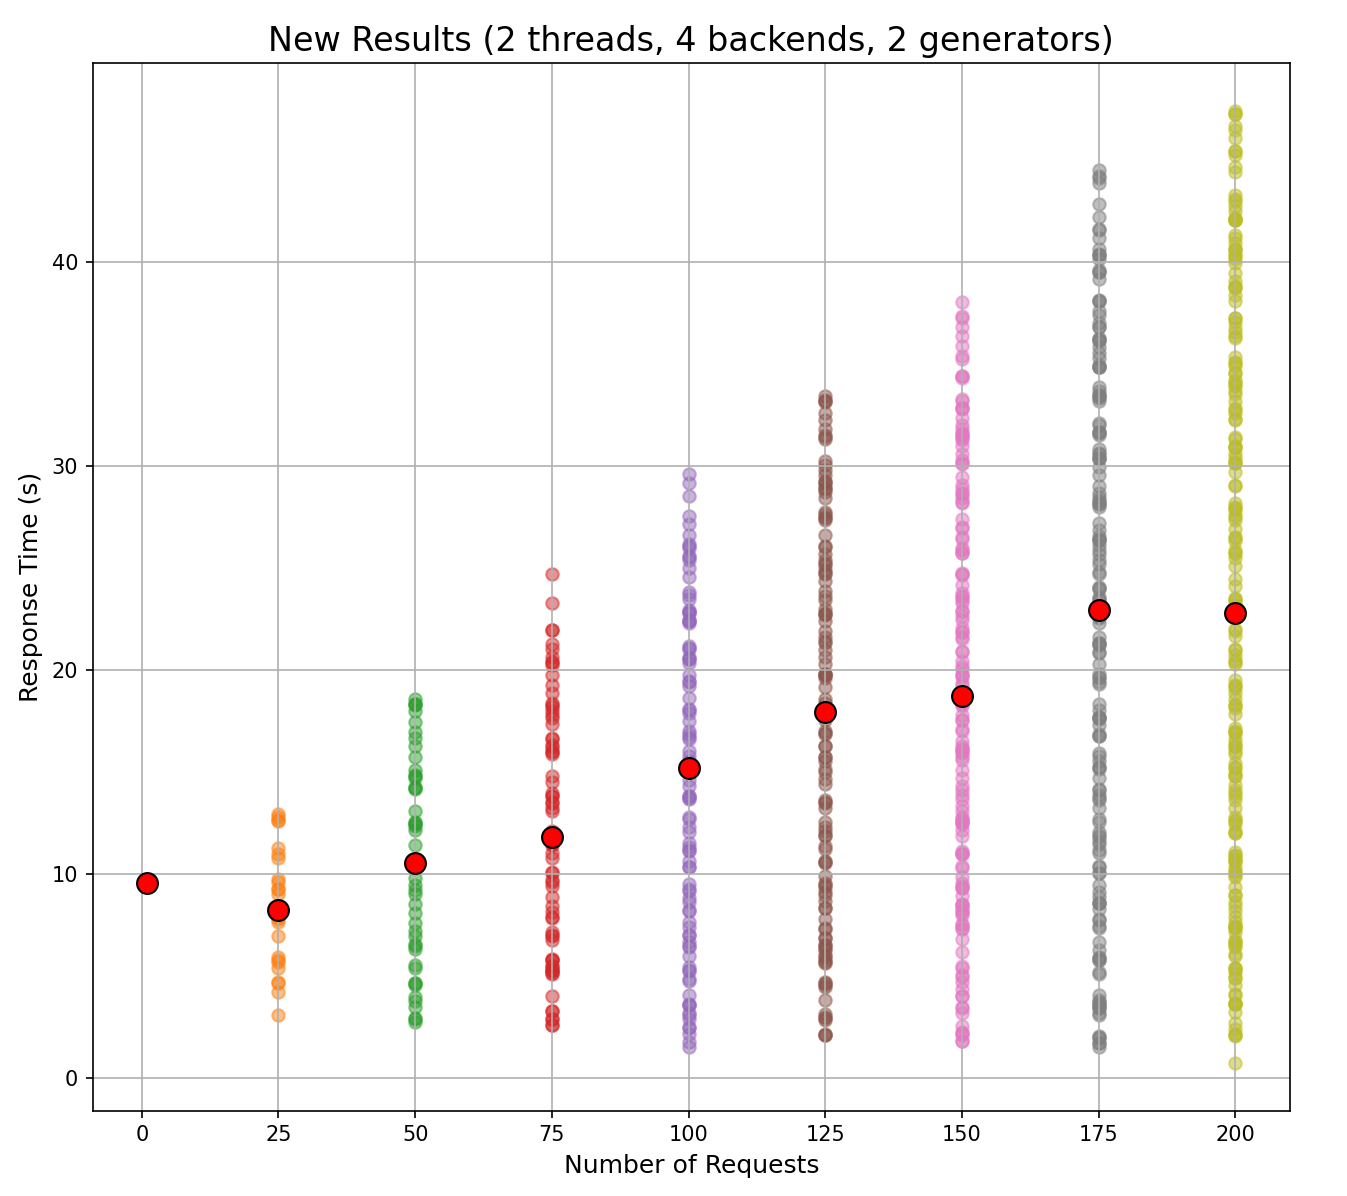
\includegraphics[scale=0.6]{include/imgs/2t_4w_2g_new.PNG}
						\caption{Generation requests with 2 threads, 4 backend instances and 2 generator instances}
						\label{2threads4web2gen}
					\end{center}
				\end{figure}

			

